\documentclass{article}
\usepackage{a4wide}
\usepackage[english]{babel}
\usepackage{amsmath}
\usepackage{amssymb}
\usepackage{dsfont}
%\usepackage[dvips]{epsfig}
%\usepackage{graphicx}
\usepackage{fancyhdr}
\usepackage{listings}
\usepackage{nomencl}
\usepackage[pdftex]{graphicx}

\usepackage{listings} 
\lstset{numbers=left, numberstyle=\tiny, numbersep=5pt} 
\lstset{language=C} 
 \lstset{basicstyle=\small}

\pagestyle{fancy}
\lhead{\footnotesize \parbox{11cm}{Andreas Johann H\"ormer (753179), Daniel Tormoen}}
\rhead{\footnotesize {Assignment 6}}
\chead{\footnotesize {TMA4280}}

\title{Report Assignment 6}
\author{Andreas Johann H\"ormer, Daniel Tormoen}
\date{\today}

\begin{document}
\thispagestyle{empty}
\maketitle
\thispagestyle{empty}
%\\[5cm]
\begin{center}
TMA4280 Supercomputing\\[3cm]
Lab group:
\begin{itemize}
\item Andreas Johann H\"ormer
\item Danny Tormoen\\[3cm]
\end{itemize}
Report delivered: 27.02.2014\\[6cm]
FACULTY OF INFORMATION TECHNOLOGY, MATHEMATICS AND ELECTRICAL ENGINEERING\\
NORWEGIAN UNIVERSITY OF SCIENCE AND TECHNOLOGY
\end{center}
\thispagestyle{empty}
\newpage
\tableofcontents
\thispagestyle{empty}
\newpage
\section*{Summary}
\thispagestyle{empty}
Matrix dimensions can get very large, so the number of matrix elements can increase quickly. So working with matrices is a perfect way to use distributed computing. In this task the matrix is transposed in the distributed system using MPI. The problem solved is a two dimensional poisson problem. The solution is done for rectangular matrices with homogeneous boundaries. As solution method diagonalization with FST is used.
\newpage
\setcounter{page}{1}
\section{Problem description}
The implementation shall solve the two-dimensional poisson problem 
\begin{equation}
-\bigtriangledown^2=f\;in\;\Omega = (0,1)x(0,1)
\end{equation}
\begin{equation}
u = 0\;on\;\delta\Omega
\end{equation}
The given poisson equation is an elliptic partial differential equation. The problem is solving this equation with given boundary conditions. 
The problem should be discretized with (n+1) points in each spatial direction. The standard 5-point-stencil to discretize the Laplace operator $\bigtriangledown$ has to be used. To obtain a solution in $O(n\cdot log(n))$ the DST should be applied.
\section{Solution strategies}
\subsection{LU factorization}
LU (lower upper) factorization decomposes a matrix in an upper and a lower triangular matrix. This can be done using Gaussian elimination. For symmetric matrizes this can also be done using the cholesky decomposition. The matrix decomposition follows following rule
\begin{equation}
A=LU
\end{equation}
where A is the original matrix, L the lower triangular matrix and U the upper triangular matrix.\\
This solution strategy is not very usable as solver in parallel contexts. The sequential nature (pivoting, substitution, ...) makes it hard for parralelization. The LU factorization needs $\mathcal{O}(n^4)$ for runtime and $\mathcal{O}(n^3)$ for memory when the matrix is sparsed, as well as $\mathcal{O}(n^6)$ Operations and $\mathcal{O}(n^4)$ memory when the matrix is full.
%Runtime O(n^4) sparsed, O(n^6) full
%Memory O(n^3) sparsed, O(n^4) full
\subsection{diagonalization}
The diagonalization can be done in three steps:
\begin{enumerate}
\item $$\underline{\tilde{B}}=\underline{Q^T}\cdot\underline{B}\cdot\underline{Q}$$
\item $$\tilde{x_{ij}}=\frac{\tilde{b_{ij}}}{\lambda_i+\lambda_j}\;for\;1\leq i,j \leq N$$
\item $$\underline{X}=\underline{Q}\cdot\underline{\tilde{X}}\cdot\underline{Q^T}$$
\end{enumerate}
This algorithm scales very well with the number of unknowns and also scales very well in memory. It is better parallelizable than LU factorization. In an further step fourier transform (DST) can be applied. The algorithm has $\mathcal{O}(n^3)$ operations and needs $\mathcal{O}(n^2)$ memory.
%O(n^3) operations
%O(n^2) memory
\subsubsection{diagonalization using DST}
For this diagonalization technique a periodic function with period $2\pi$ is sampled at equidistant points. The function has to be odd and discretized on a equidistant mesh between 0 and $\pi$.The diagonalization can be done in the three following steps:
\begin{enumerate}
\item $$ \underline{\tilde{B}^T}=\underline{S^{-1}}\cdot\big((\underline{S}\cdot\underline{B})^T\big)$$
\item $$ \tilde{x_{ij}}=\frac{\tilde{b_{ij}}}{\lambda_i+\lambda_j}\;for\;1\leq i,j\leq N$$
\item $$ \underline{X}=\underline{S^{-1}}\cdot\big(\underline{S}\cdot(\underline{\tilde{X^T}})\big)^T$$
\end{enumerate}
\section{Implemented solution}
\subsection{matrix transpose}
The matrix is transposed using the message passing interface. This is done using MPI\_Alltoallv(). A code sample for doing this can be seen in section \ref{matrixtranspose}.
\section{Environment}
\subsection{Supercomputer}
The used Kongull cluster is a CentOS 5.3 Linux cluster. The cluster has 1 login, 4 I/O and 93 compute nodes. Each node is equipped with 2x 6-core processors, with 6x 512KiB L1 cache and a common 6 MiB L3-cache. Kongull has 96 compute nodes and 1152 cores in total. All of the compute nodes are HP DL165 G6 servers, with
\begin{itemize}
\item 2 AMD Opteron model 2431 6-core (Istanbul) processors
\item 2.4 GHz core speed
\item 667 MHz (48 GiB nodes) or 800 MHz (24 GiB nodes) bus frequency
\item 149GiB 15000 RPM SAS system disc
\end{itemize}
This and further information about the used supercomputer can be found at the NTNU HPC homepage\footnote{https://www.hpc.ntnu.no/display/hpc/Kongull+Hardware, accessed: 18.03.2014}.
\subsection{Compiler}

For our solution we used following packages on kongull:
\begin{itemize}
\item intelcomp13.0.1
\item openmpi1.4.3-intel
\end{itemize}
\section{Results}
\subsection{Proof of Correctness}
	To verify the correctness of our method we used a series of tests to ensure each part of the algorithm is producing the results we expect. When we completed the transpose function we tested the transpose function for a variety of sizes and number of MPI processes to ensure that the function was producing the correct matrix. 

	Before we started work on the OpenMP parallelization we tried the complete algorithm with our own function that we knew the exact solution to. We then compared the numeric estimate our program produces to the exact solution to see if they converge. The initial values in each grid location are given by equation \ref{eqn:gridInitial}.

	\begin{equation}
		\label{eqn:gridInitial}
		f(x,y) = 5\pi^2 \sin(\pi x)* \sin(2\pi y)
	\end{equation}

	Equation \ref{eqn:gridExact} shows the exact solution for a grid point. We can find the maximum error at each grid point by taking the absolute value of the difference between the estimate for the grid point and the exact solution. We keep track of the maximum error for any grid point as a measurement of the error.

	\begin{equation}
		\label{eqn:gridExact}
		u(x,y) = \sin(\pi x) * \sin(2 \pi y)
	\end{equation}

	Using this method the maximum error should decrease by a factor of 4 every time we increase the number of grid points in a row by a factor of 2. Assume $e$ is the maximum error for a poisson numerical estimation of size $n \times n$. The error $e$ is given by \ref{eqn:error}.

	\begin{equation}
		\label{eqn:error}
		e = \Theta(\frac{1}{n^2})
	\end{equation}

	

\section{Analysis}
%\begin{figure}[htbp]
%\begin{center}
%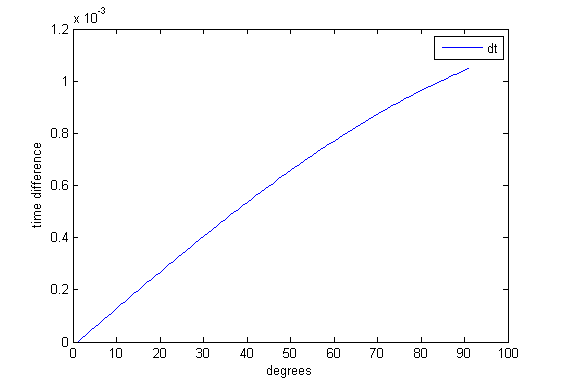
\includegraphics[width=15cm,keepaspectratio=true]{angles}
%\caption{Time differences for sound signal at two ears}
%\label{fig:angles}
%\end{center}
%\end{figure}



\section{Possible optimizations}
\subsection{parallel FST}
In our algorithm the FST is serial. This could be a possible bottleneck.
\subsection{rectangular matrix}
Our algorithm is designed for handling squared matrizes with zero-boundary. For handling rectangular matrices this can be done with following:
\begin{equation}
-U_0+2U_1-U_2=h^2f_1
\end{equation}
When moving $U_0$ to the other side and writing in a general form this changes to
\begin{equation}
-U_{N-2}+2U_{N-1}-U_N=h^2f_{N-1}
\end{equation}
For rectangular matrices the sizing in x- and y-direction is different. So the multiplication is done with two different variables, $h_x$ and $h_y$.
\begin{equation}
\frac{1}{h_x^2}A_DU+\frac{1}{h_y^2}UA_D=F
\end{equation}
The matrix which is added on the right side looks then
$$
\begin{bmatrix}
U_{1,1} & U_{2,1} & 0 & ... & 0 & U_{N_x-1,1} & U_{N_x,1} \\
U_{1,2} & 0 & ... & ... & ... & 0 & U_{N_x,2} \\
... & ... & ... & ... &... & ... & ... \\
U_{1,N_y} & U_{2,N_y} & 0 & ... & 0 & U_{N_x-1,N_y} & U_{N_x,N_y} 
\end{bmatrix}
$$
\subsection{non-homogeneus boundary conditions}
This optimization can be done in a similiar way like the rectangular matrices. The boundary has to be moved to the right side which looks like the rectangular matrix. The calculation can be done using following formula
\begin{equation}
\frac{G_{i,j}}{\frac{1}{\sqrt{h_x^2}}\lambda_i+\frac{1}{\sqrt{h_x^2}}\lambda_j}
\end{equation}
%parallel fst
%not much possibilities
\newpage
\section{Conclusion}

\section{Appendix}
\subsection{Code samples}
\subsubsection{Matrix transpose\label{matrixtranspose}}
\begin{lstlisting}[caption=Matrix transposition using MPI]{Matrix transpose}
    for(rowcnt=0; rowcnt<m; rowcnt++)
    {
        for(columncnt=0; columncnt<scnt[rank]; columncnt++)
        {
            sendvector[vectorposition]=b[columncnt][rowcnt];
            vectorposition++;
        }
    }
    MPI_Alltoallv (
        sendvector,	MPIscnt, MPIdispl, MPI_DOUBLE, receivevector,
        MPIscnt, MPIdispl, MPI_DOUBLE, MPI_COMM_WORLD);
  for (proccnt = 0; proccnt < size; ++proccnt)
    {
        for(columncnt=0; columncnt<scnt[rank];columncnt++)
        {
            for (rowcnt = displ[proccnt]; 
		rowcnt < displ[proccnt] + scnt[proccnt]; ++rowcnt)
            {

                bt[columncnt][rowcnt]=receivevector[vectorposition];
                vectorposition++;
            }
        }
    }
\end{lstlisting}
Description: hmmm
\end{document}
